% Options for packages loaded elsewhere
\PassOptionsToPackage{unicode}{hyperref}
\PassOptionsToPackage{hyphens}{url}
%
\documentclass[
  ignorenonframetext,
]{beamer}
\usepackage{pgfpages}
\setbeamertemplate{caption}[numbered]
\setbeamertemplate{caption label separator}{: }
\setbeamercolor{caption name}{fg=normal text.fg}
\beamertemplatenavigationsymbolsempty
% Prevent slide breaks in the middle of a paragraph
\widowpenalties 1 10000
\raggedbottom
\setbeamertemplate{part page}{
  \centering
  \begin{beamercolorbox}[sep=16pt,center]{part title}
    \usebeamerfont{part title}\insertpart\par
  \end{beamercolorbox}
}
\setbeamertemplate{section page}{
  \centering
  \begin{beamercolorbox}[sep=12pt,center]{part title}
    \usebeamerfont{section title}\insertsection\par
  \end{beamercolorbox}
}
\setbeamertemplate{subsection page}{
  \centering
  \begin{beamercolorbox}[sep=8pt,center]{part title}
    \usebeamerfont{subsection title}\insertsubsection\par
  \end{beamercolorbox}
}
\AtBeginPart{
  \frame{\partpage}
}
\AtBeginSection{
  \ifbibliography
  \else
    \frame{\sectionpage}
  \fi
}
\AtBeginSubsection{
  \frame{\subsectionpage}
}
\usepackage{amsmath,amssymb}
\usepackage{iftex}
\ifPDFTeX
  \usepackage[T1]{fontenc}
  \usepackage[utf8]{inputenc}
  \usepackage{textcomp} % provide euro and other symbols
\else % if luatex or xetex
  \usepackage{unicode-math} % this also loads fontspec
  \defaultfontfeatures{Scale=MatchLowercase}
  \defaultfontfeatures[\rmfamily]{Ligatures=TeX,Scale=1}
\fi
\usepackage{lmodern}
\ifPDFTeX\else
  % xetex/luatex font selection
\fi
% Use upquote if available, for straight quotes in verbatim environments
\IfFileExists{upquote.sty}{\usepackage{upquote}}{}
\IfFileExists{microtype.sty}{% use microtype if available
  \usepackage[]{microtype}
  \UseMicrotypeSet[protrusion]{basicmath} % disable protrusion for tt fonts
}{}
\makeatletter
\@ifundefined{KOMAClassName}{% if non-KOMA class
  \IfFileExists{parskip.sty}{%
    \usepackage{parskip}
  }{% else
    \setlength{\parindent}{0pt}
    \setlength{\parskip}{6pt plus 2pt minus 1pt}}
}{% if KOMA class
  \KOMAoptions{parskip=half}}
\makeatother
\usepackage{xcolor}
\newif\ifbibliography
\usepackage{graphicx}
\makeatletter
\def\maxwidth{\ifdim\Gin@nat@width>\linewidth\linewidth\else\Gin@nat@width\fi}
\def\maxheight{\ifdim\Gin@nat@height>\textheight\textheight\else\Gin@nat@height\fi}
\makeatother
% Scale images if necessary, so that they will not overflow the page
% margins by default, and it is still possible to overwrite the defaults
% using explicit options in \includegraphics[width, height, ...]{}
\setkeys{Gin}{width=\maxwidth,height=\maxheight,keepaspectratio}
% Set default figure placement to htbp
\makeatletter
\def\fps@figure{htbp}
\makeatother
\setlength{\emergencystretch}{3em} % prevent overfull lines
\providecommand{\tightlist}{%
  \setlength{\itemsep}{0pt}\setlength{\parskip}{0pt}}
\setcounter{secnumdepth}{-\maxdimen} % remove section numbering
\ifLuaTeX
  \usepackage{selnolig}  % disable illegal ligatures
\fi
\usepackage{bookmark}
\IfFileExists{xurl.sty}{\usepackage{xurl}}{} % add URL line breaks if available
\urlstyle{same}
\hypersetup{
  pdftitle={Untitled},
  pdfauthor={Son Nguyen},
  hidelinks,
  pdfcreator={LaTeX via pandoc}}

\title{Untitled}
\author{Son Nguyen}
\date{2024-09-17}

\begin{document}
\frame{\titlepage}

\begin{frame}{Reading Materials}
\phantomsection\label{reading-materials}
\begin{itemize}
\tightlist
\item
  Max Kuhn. Chapter 14. Section 14.1
\end{itemize}
\end{frame}

\begin{frame}{Decision Boundary in Classification}
\phantomsection\label{decision-boundary-in-classification}
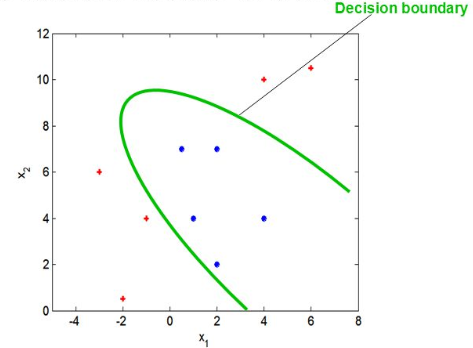
\includegraphics{images/db.png}

Classification is a process of finding the \textbf{decision boundary}
that best separate two classes
\end{frame}

\begin{frame}{Decision Boundary in Classification}
\phantomsection\label{decision-boundary-in-classification-1}
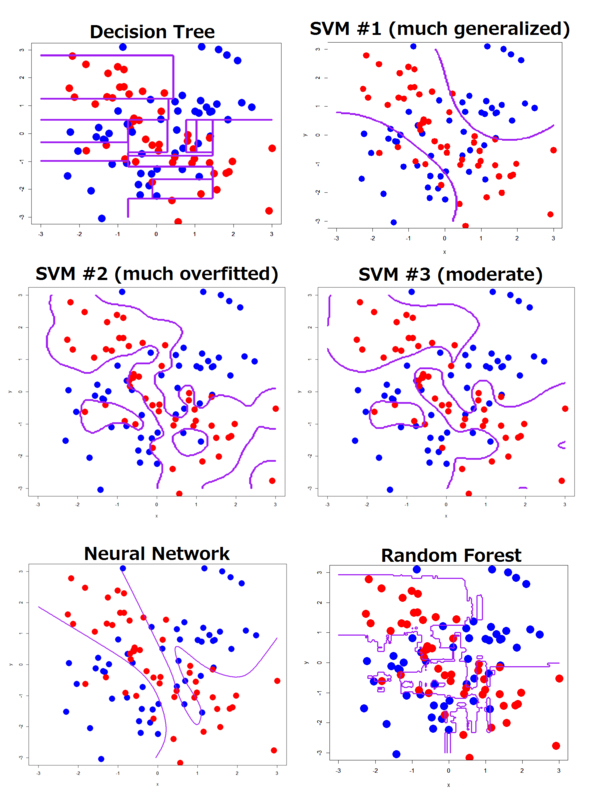
\includegraphics{images/db1.png}

SVM = Support Vector Machine
\end{frame}

\begin{frame}{Decision Tree}
\phantomsection\label{decision-tree}
\begin{itemize}
\tightlist
\item
  Decision Tree for classification is \textbf{Classification Tree}
\item
  Decision Tree for Regression is \textbf{Regression Tree}
\end{itemize}
\end{frame}

\begin{frame}{Example of Classification Tree}
\phantomsection\label{example-of-classification-tree}
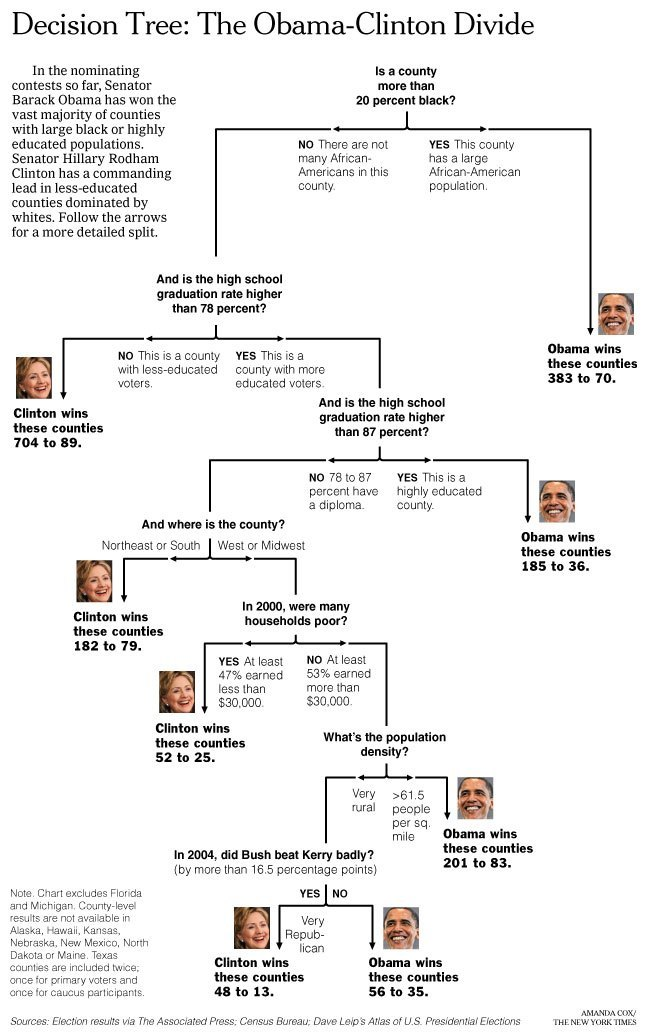
\includegraphics{images/tree2.jpg}

{[}Link{]}
(\url{http://graphics8.nytimes.com/images/2008/04/16/us/0416-nat-subOBAMA.jpg})
\end{frame}

\begin{frame}{Classification Tree}
\phantomsection\label{classification-tree}
\begin{itemize}
\tightlist
\item
  In two dimension, classification Tree's decision boundary is a
  collection of horizontal and vertical line
\end{itemize}
\end{frame}

\begin{frame}{Data}
\phantomsection\label{data}
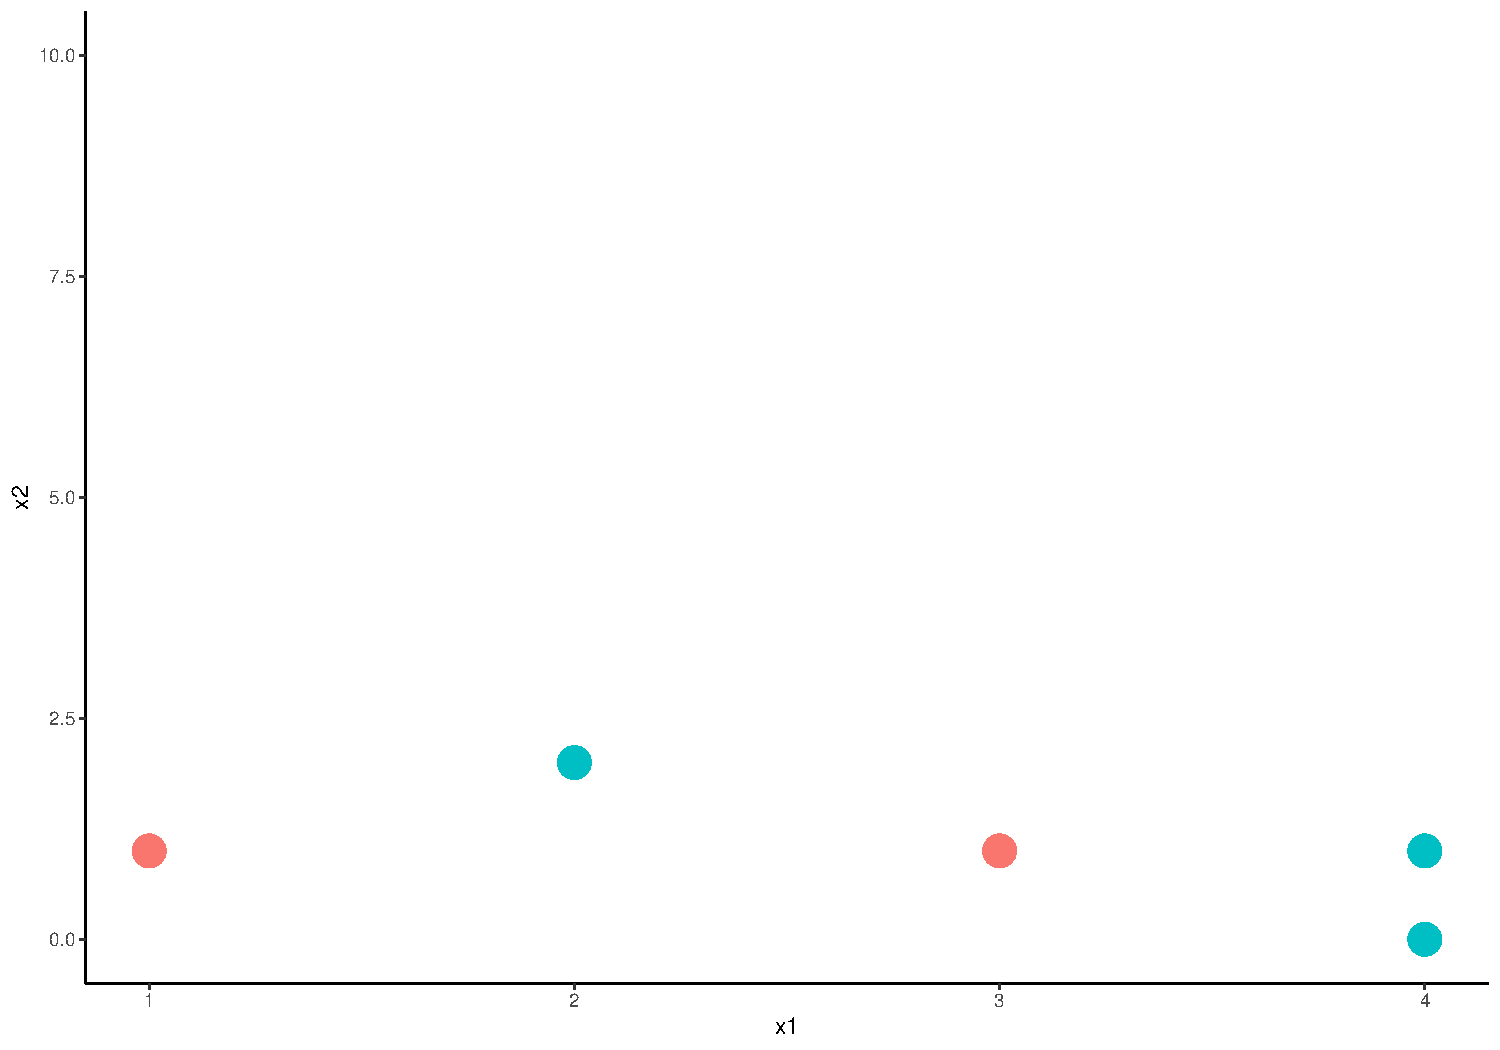
\includegraphics{fall24_classification_tree_remake_files/figure-beamer/unnamed-chunk-1-1.pdf}

\begin{itemize}
\tightlist
\item
  The tree starts by a vertical or horizontal line that \textbf{best}
  seperate the data
\item
  \textbf{Question}: Find a vertical line that best seperate
  \textbf{red} and \textbf{green}.
\end{itemize}
\end{frame}

\begin{frame}[fragile]{One way to seperate the reds and greens}
\phantomsection\label{one-way-to-seperate-the-reds-and-greens}
\begin{verbatim}
## Warning: Using `size` aesthetic for lines was deprecated in ggplot2 3.4.0.
## i Please use `linewidth` instead.
## This warning is displayed once every 8 hours.
## Call `lifecycle::last_lifecycle_warnings()` to see where this warning was
## generated.
\end{verbatim}

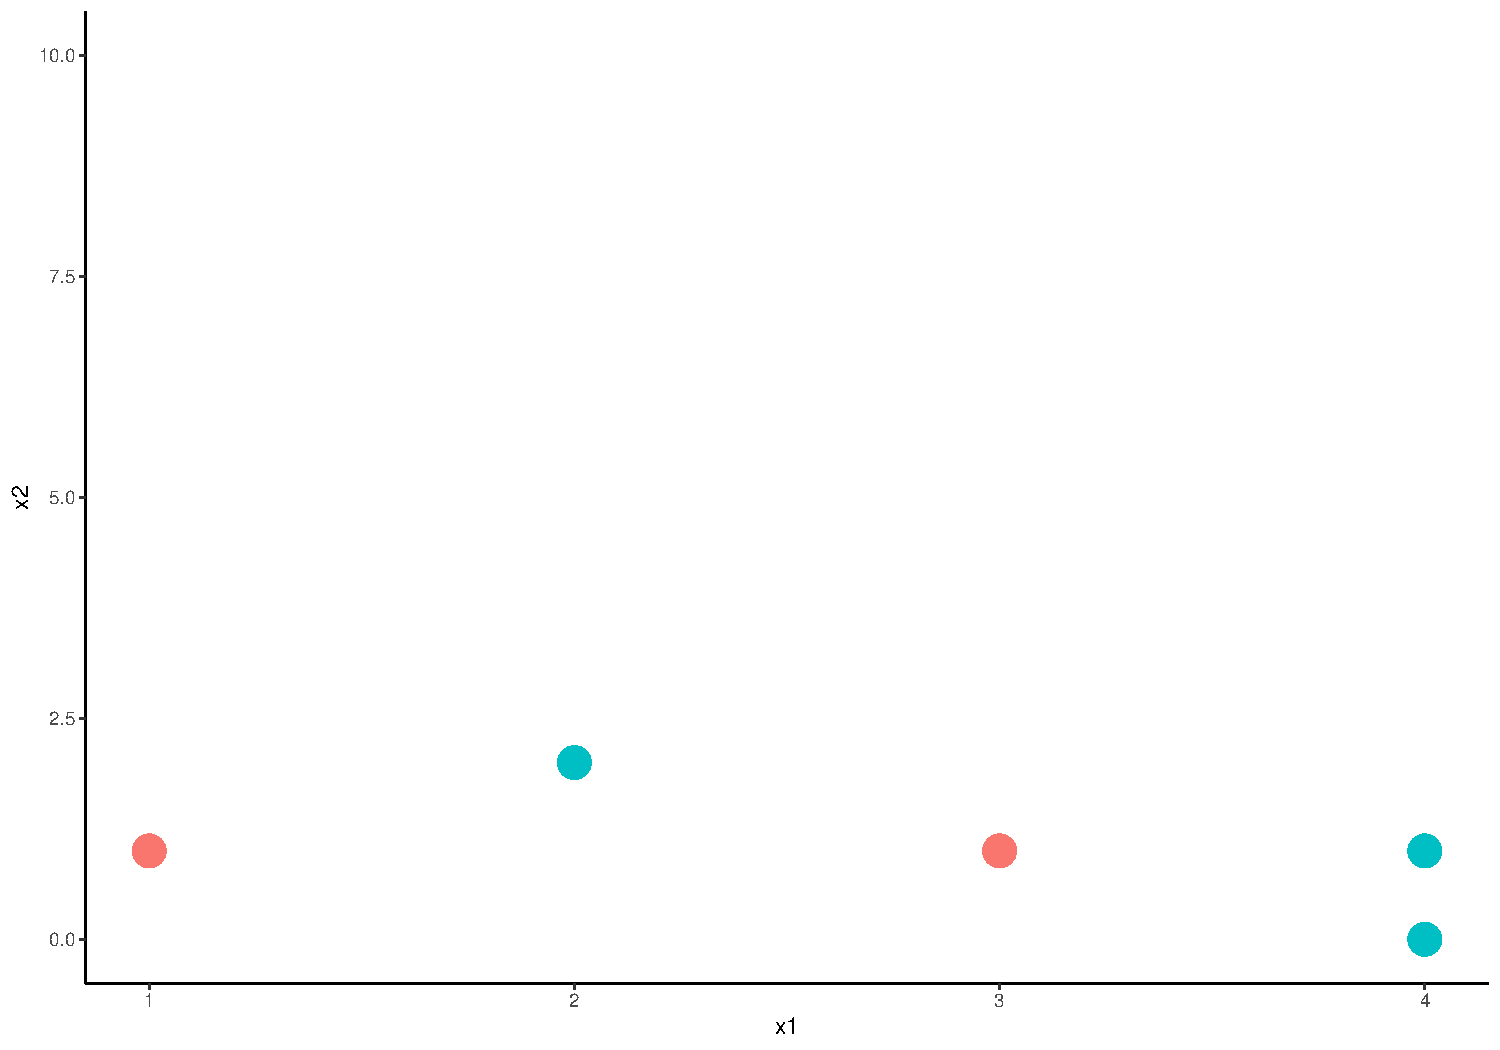
\includegraphics{fall24_classification_tree_remake_files/figure-beamer/unnamed-chunk-2-1.pdf}
\end{frame}

\begin{frame}{One way to seperate the reds and greens}
\phantomsection\label{one-way-to-seperate-the-reds-and-greens-1}
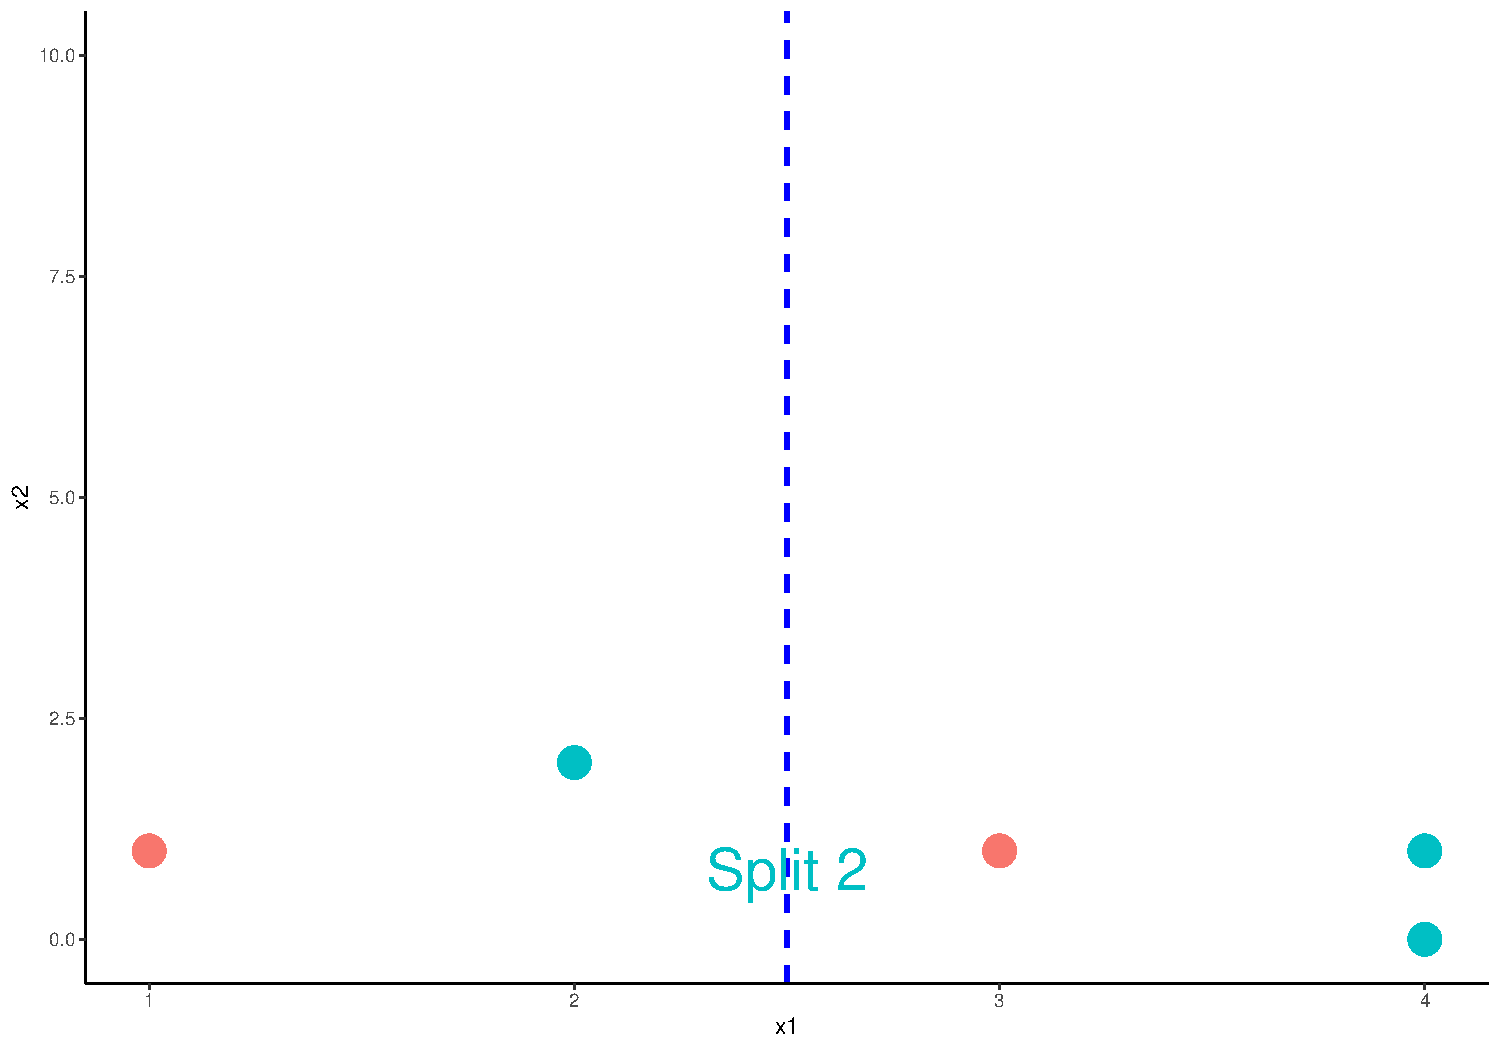
\includegraphics{fall24_classification_tree_remake_files/figure-beamer/unnamed-chunk-3-1.pdf}
\end{frame}

\begin{frame}{One way to seperate the reds and greens}
\phantomsection\label{one-way-to-seperate-the-reds-and-greens-2}
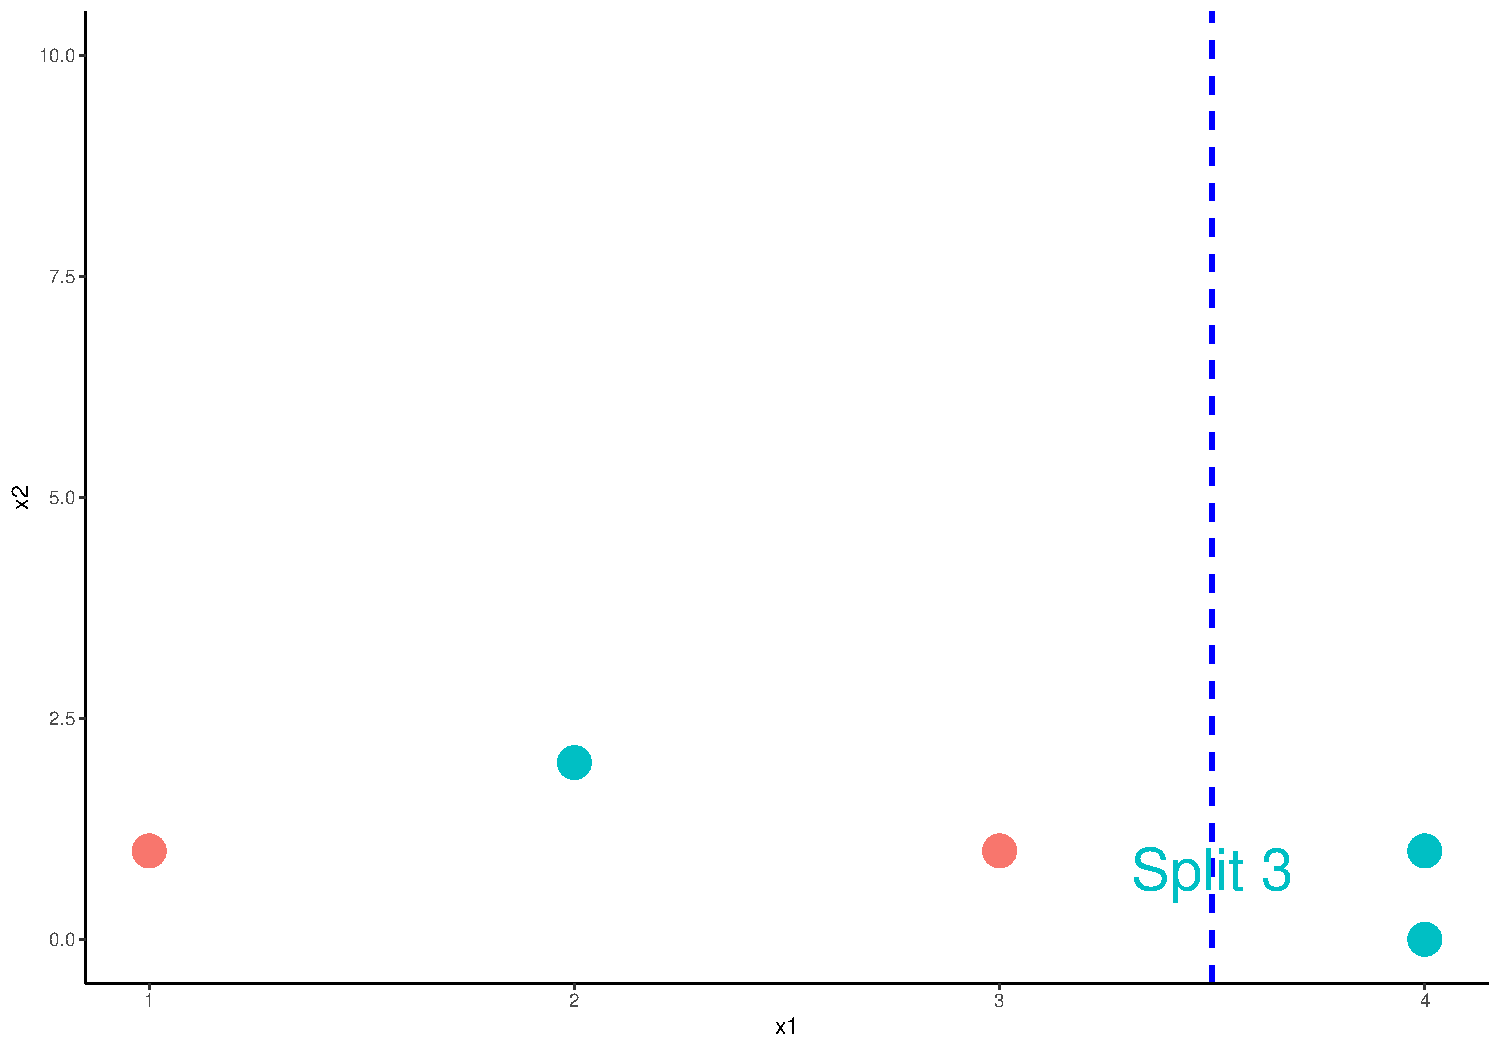
\includegraphics{fall24_classification_tree_remake_files/figure-beamer/unnamed-chunk-4-1.pdf}
\end{frame}

\begin{frame}{Question}
\phantomsection\label{question}
\begin{itemize}
\tightlist
\item
  \textbf{Question}: Which is the best split?
\end{itemize}
\end{frame}

\begin{frame}{Partial Answer}
\phantomsection\label{partial-answer}
\begin{itemize}
\tightlist
\item
  It looks like Split 1 and 3 are better than Split 2 since it
  misclassifies less
\item
  Which is the better split between Split 1 and Split 3?
\item
  We need to find a way to measure \emph{how good a split is}
\end{itemize}
\end{frame}

\begin{frame}{Impurity Measure}
\phantomsection\label{impurity-measure}
\begin{itemize}
\tightlist
\item
  The impurity of a node (\textbf{a node = a subset of the data or the
  original data}) measure how uncertain the node is.\\
\item
  For example, node A with 50\% reds and 50\% greens would be more
  uncertained than node B with 90\% reds and 10\% greens. Thus, node A
  has greater impurity than node B.
\item
  More uncertained \(=\) Greater impurity
\end{itemize}
\end{frame}

\begin{frame}{Impurity Measure}
\phantomsection\label{impurity-measure-1}
\begin{itemize}
\tightlist
\item
  A split that \emph{gains} more impurity is the \textbf{better split}!
\end{itemize}
\end{frame}

\begin{frame}{Impurity Gain}
\phantomsection\label{impurity-gain}
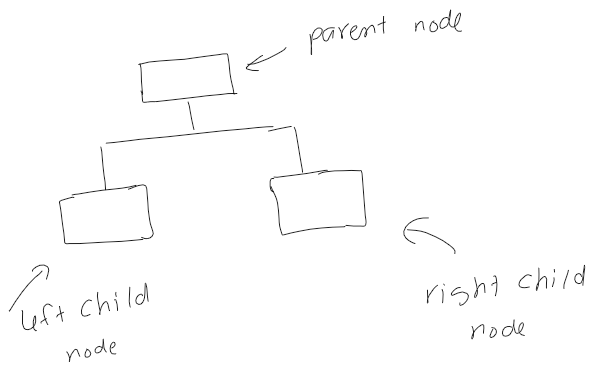
\includegraphics{images/parent_child.png}

\[
IG = I_{parent} - \frac{N_{left}}{N}I_{left}-\frac{N_{right}}{N}I_{right}
\]

\begin{itemize}
\tightlist
\item
  IG is Impurity Gain of the split
\item
  \(N_{left}\) and \(N_{right}\) are the number of points in the left
  child node and right child node, respectively.
\item
  \(N_{left}+N_{right}=N\)
\end{itemize}
\end{frame}

\begin{frame}{Impurity Measure}
\phantomsection\label{impurity-measure-2}
\begin{itemize}
\tightlist
\item
  Impurity can be measured by: classification error, Gini Index, and
  Entropy.
\end{itemize}
\end{frame}

\begin{frame}{Impurity Measure}
\phantomsection\label{impurity-measure-3}
\begin{itemize}
\tightlist
\item
  Let \(p_0\) and \(p_1\) be the proportion of class 0 and class 1 in a
  node.
\end{itemize}

\begin{align*}
{\text{By Classification Error: }} I &= min\{p_0, p_1\} \\
{\text{By Gini Index: }} I&= 1 - p_0^2-p_1^2 \\
{\text{By Entropy: }} I &= -p_0 \log_2(p_0)-p_1\log_2(p_1) 
\end{align*}
\end{frame}

\end{document}
